\documentclass[conference]{IEEEtran}

\usepackage{amsmath,amssymb}
\usepackage{graphicx}
\usepackage{booktabs}
\usepackage{multirow}
\usepackage{cite}
\usepackage{url}
\usepackage{xcolor}
\usepackage{array}
\usepackage{tabularx}
\usepackage{balance}

\begin{document}

\title{Auditable Mixed-Precision Deployment of Prithvi-EO-2.0 on a K100 AI Accelerator: Accuracy, Kernel Paths, and System Trade-offs}

\author{\IEEEauthorblockN{Anonymous Author(s)}
\IEEEauthorblockA{Anonymous Institution\\Anonymous Location\\anonymous@example.com}}

\maketitle

\begin{abstract}
Deploying geospatial foundation models requires evidence beyond nominal datatype and file compression. We present an auditable, hardware- and runtime-specific case study of a 319M-parameter Prithvi-EO-2.0-300M model with a UPerNet decoder for flood-water segmentation on a K100 AI accelerator. The validation chain covers task utility on a fixed 90-image split, ONNX Runtime Execution Provider placement, realized GEMM kernel paths, topology-matched and same-CLI performance, and operational behavior of immutable bundles. A 25-segment FP32 denominator and six fixed diagnosis-informed FP16/INT8 configurations (M0--M5) are evaluated. M4 has the highest measured mixed-precision mIoU (0.86037), while M5 obtains 0.86027 mIoU and a 22.080 ms end-to-end-logits median, approximately 0.58\% below the 22.209 ms segmented-FP32 median; this is treated as latency parity, not a formal INT8 speedup. Profiles contain positive MIGraphX and zero CPU provider events, and traces identify I8II GEMMs in retained INT8 blocks and HBH GEMMs in FP16 blocks. Under a production-style same-CLI comparison, however, M5 is 73.642\% slower than the monolithic Full FP16 bundle, although its complete payload is 23.463\% smaller. Both bundles pass five cold starts, three forced-restart recoveries, two-node smoke tests, and 60-minute stability runs without inference errors, non-finite outputs, or prediction drift. For the evaluated checkpoint and K100 software stack, Full FP16 is the speed-oriented primary deployment and M5 is a storage-oriented deployable alternative.
\end{abstract}

\begin{IEEEkeywords}
geospatial foundation model, mixed precision, deployment validation, MIGraphX, K100
\end{IEEEkeywords}

\section{Introduction}
\label{sec:introduction}

Geospatial foundation models (GeoFMs) transfer large-scale pre-training to downstream Earth-observation tasks such as land-cover mapping, change detection, and disaster response. Prithvi-EO-2.0 extends this direction with multi-temporal and location-aware pre-training over Harmonized Landsat and Sentinel-2 imagery~\cite{prithvi2024}. Related masked-autoencoding models exploit the temporal and spectral structure of satellite imagery~\cite{satmae2022}. Their downstream graphs can nevertheless contain hundreds of millions of parameters, normalization and attention operators, multi-scale feature reconstruction, and dense prediction heads.

Low-precision inference can reduce artifact capacity and may expose low-precision kernels. Yet task preservation, accelerator placement, realized arithmetic, and application latency are distinct claims. Vision-Transformer post-training quantization (PTQ) addresses activation distributions, LayerNorm variation, and reparameterization~\cite{ptq4vit2022,fqvit2022,repqvit2023}, while hardware-aware mixed precision emphasizes the cost of conversions and runtime constraints~\cite{hawqv3}. Compiler fusion, graph partitioning, Q/DQ boundaries, layout conversion, and session scheduling can therefore offset nominal arithmetic savings.

This work studies Prithvi-EO-2.0-300M with UPerNet~\cite{upernet2018} on the K100 AI accelerator. \emph{This work does not propose a new quantization algorithm or a universally transferable mixed-precision policy.} It is a hardware- and runtime-specific deployment case study. We preserve the failed strict CPU/MIGraphX logit diagnostic, but use a separately defined application-level track to examine whether an immutable artifact is usable on the target stack. The evidence is organized into five layers: task utility, provider placement, realized kernels, system performance, and operations.

Our main contributions are:
\begin{enumerate}
    \item We define an auditable five-layer evidence framework that separates task utility, provider placement, realized kernels, performance, and operational reliability rather than treating nominal INT8 or compression as deployment success.
    \item We establish a topology-matched 25-segment FP32 denominator with device-resident inter-segment OrtValues, making the segmented M0--M5 timing comparison explicit and reproducible.
    \item We map immutable ONNX configurations to provider profiles and block-level I8II/HBH traces: 33 de-duplicated artifact traces support 144 candidate--block mappings, with no profiled CPU provider events.
    \item We package M5 and Full FP16 as immutable bundles and validate cold start, forced recovery, cross-node execution, 60-minute operation, and a production-style same-CLI comparison.
\end{enumerate}

We make no claim that all operators in the mixed graph are native INT8, that strict CPU/MIGraphX logits are equivalent, or that INT8 arithmetic necessarily accelerates the complete application.

\section{Related Work}
\label{sec:related_work}

\subsection{Geospatial Foundation Models and Downstream Adaptation}

Vision Transformers (ViTs) apply self-attention to patch sequences~\cite{vit2021}. Remote-sensing masked pre-training has subsequently incorporated temporal and multispectral inputs, explicit spatial scale, and aligned radar--optical data, as illustrated by SatMAE, Scale-MAE, and CROMA~\cite{satmae2022,scalemae2023,croma2023}. RingMo and continual geospatial pre-training broaden the learned representations across sensors and downstream tasks~\cite{ringmo2023,gfm2023}, while SkySense and DOFA address multimodal or sensor-flexible Earth-observation encoders~\cite{skysense2024,dofa2024}. Prithvi-EO-2.0 focuses on multitemporal, location-aware pre-training and downstream adaptation~\cite{prithvi2024}. These studies establish transferable representations; they do not by themselves resolve the target-runtime behavior of a dense-prediction deployment.

\subsection{Post-Training Quantization and Mixed Precision for Transformers}

Integer inference can reduce model size and execute integer arithmetic when quantization semantics and kernels align~\cite{jacob2018}. Vision-Transformer PTQ methods study ranking-preserving calibration, non-Gaussian activations, LayerNorm variation, and scale reparameterization~\cite{vitptq2021,ptq4vit2022,fqvit2022,repqvit2023}. Hardware-aware and sensitivity-aware mixed-precision methods allocate bit widths using device feedback or layer-level signals~\cite{haq2019,hawqv3,mixqvit2026}. Our work neither introduces a PTQ formulation nor estimates task-loss sensitivity. It examines fixed precision maps informed by discrepancies observed between two backends executing the same frozen artifacts.

\subsection{Hardware-Aware Deployment and Runtime Compilation}

ONNX Runtime exposes an Execution Provider abstraction for framework-exported graphs~\cite{onnxruntime}; MIGraphX compiles and lowers supported operations to target kernels~\cite{migraphx}. Reproducible inference benchmarking also requires explicit scenarios, accuracy constraints, and timing definitions rather than a single unqualified latency value~\cite{mlperf2020}. Provider registration alone does not establish node placement, and node placement does not identify the realized GEMM datatype. We therefore connect model identity, provider profiles, kernel traces, and matched latency rather than using graph datatype as a performance proxy.

\subsection{Deployment Validation for Remote-Sensing Models}

Remote-sensing compression studies increasingly consider model size together with resolution and accuracy~\cite{shinde2025}. Operational work also stresses application requirements, domain adaptation, and empirical validation outside a benchmark-only view~\cite{worldcereal2025}. PhiSat-1 provides an example of on-board deep-learning validation under a constrained Earth-observation setting~\cite{phisat2022}, and a recent review organizes onboard remote-sensing foundation-model deployment around model optimization, software toolchains, and resource-constrained hardware~\cite{sang2026}. These studies motivate a deployment view in which an artifact must be executable, measurable, and recoverable, not merely accurate in an offline framework.

Among the studies reviewed in this work, we did not identify a single evaluation chain that jointly reports task utility, provider placement, realized kernels, topology-matched performance, and operational behavior on a target GeoFM stack. This case study reports those evidence layers together while limiting its conclusions to the evaluated checkpoint and K100 software stack.

\section{Model and Deployment Method}
\label{sec:method}

Deployment proceeds from the frozen FP32 reference through backend-discrepancy diagnosis and fixed precision configurations to K100 execution. The evidence path keeps task utility, provider placement, realized kernels, system performance, and operational acceptance separate.

Figure~\ref{fig:framework} summarizes the immutable-artifact pipeline and the five evidence layers used to reach the deployment decision. The diagram is an audit structure, not a new quantization algorithm: file precision, provider placement, realized kernel precision, system performance, and operational reliability remain distinct claims.

\begin{figure*}[t]
\centering
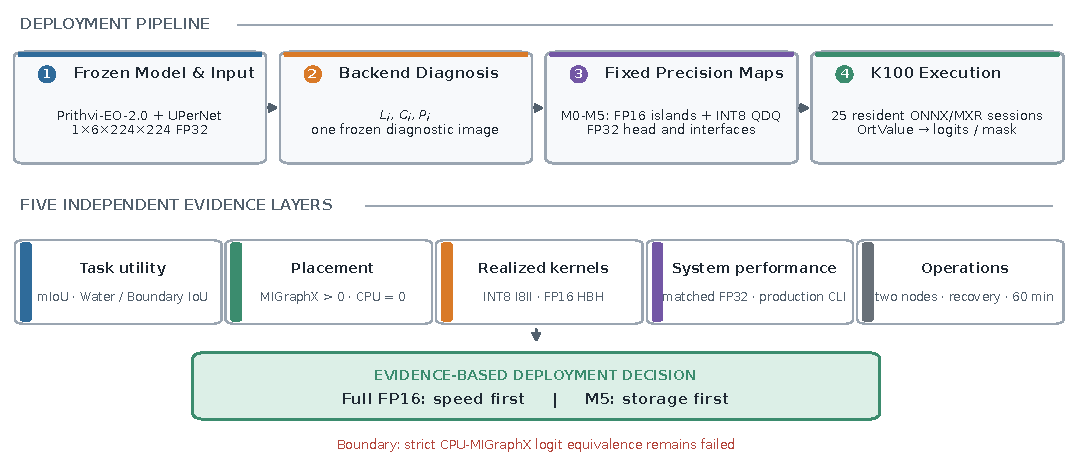
\includegraphics[width=0.98\textwidth]{figures/fig1_k100_framework_en.pdf}
\caption{Auditable K100 deployment overview. Frozen model and input identities flow through backend diagnosis, fixed M0--M5 precision maps, and 25 resident ONNX/MXR sessions. Immutable artifacts and the five evidence layers remain separate; the final engineering decision is not inferred from nominal datatype alone.}
\label{fig:framework}
\end{figure*}

\subsection{Task and Frozen Input Contract}

The task is binary flood-water segmentation on Sen1Floods11~\cite{sen1floods11}. The model combines the Prithvi-EO-2.0-300M encoder with a UPerNet decoder and contains approximately 319M parameters. Evaluation uses the fixed public test split of 90 images and 3,927,398 valid pixels. Each input has shape $1\times6\times224\times224$ and contains the bands BLUE, GREEN, RED, NIR\_NARROW, SWIR\_1, and SWIR\_2 in this order. Inputs are finite FP32 reflectance tensors after the dataset scale factor of $10^{-4}$; normalization is embedded in the exported model and is not repeated by the deployment client.

We report global confusion-matrix metrics: mean intersection-over-union (mIoU), Water IoU, pixel accuracy, and Boundary Water IoU. For a binary water mask $m$, the implementation forms a two-pixel-radius morphological gradient
\begin{equation}
\begin{aligned}
B(m)&=\delta_{2}(m)-\left[1-\delta_{2}(1-m)\right],\\
\operatorname{BIoU}&=\frac{|B(\hat m)\cap B(m)\cap V|}{|(B(\hat m)\cup B(m))\cap V|},
\end{aligned}
\label{eq:boundary-iou}
\end{equation}
where $\delta_{2}$ is max pooling with a $5\times5$ square kernel and unit stride, water is class 1, and $V$ is the target-not-ignore mask. Intersection and union are accumulated globally over all 90 images; an empty global union is reported as undefined rather than assigned an artificial score. The qualifier ``corrected'' in earlier artifacts denotes a repaired implementation that inserts the singleton channel dimension before masking, avoiding an erroneous $N\times N\times H\times W$ broadcast; throughout this paper the metric is simply called Boundary Water IoU. The application-level acceptance criteria relative to frozen FP32 are: mIoU degradation no greater than 0.5 percentage points (pp), Water IoU and Boundary Water IoU degradation no greater than 1.0 pp, valid-pixel prediction agreement of at least 99.5\%, and no non-finite outputs.

\subsection{Twenty-Five-Segment Execution Topology}

The deployed backbone is represented as 24 Transformer-block segments followed by one UPerNet head segment. All inter-segment interfaces are FP32 and use device-resident ONNX Runtime OrtValues, preventing host staging between adjacent segments. LayerNorm is expanded where required by the target compiler; decoder ConvTranspose operations are rewritten; and an fpn4 MaxPool barrier is used in the head to obtain stable accelerator placement. Each segment has an immutable ONNX identity and a compiled MXR cache identity.

The same topology is applied to FP32 and the mixed candidates. This matters because a monolithic FP32 session and a 25-session mixed pipeline have different scheduling and caching costs. The 25-segment FP32 baseline is therefore the denominator for topology-matched comparisons.

\subsection{Backend-Discrepancy Localization}

The configuration sequence was informed by an explicit segmentwise backend diagnosis rather than final logits alone. For segment $i$, let $x_i^{C}$ be the input produced by the CPU reference chain, $x_i^{M}$ the input produced by the cumulative MIGraphX chain, and $f_i^{C}$ and $f_i^{M}$ the CPU and MIGraphX executions of the same frozen segment artifact. We compute three complementary discrepancies:
\begin{equation}
\begin{aligned}
L_i &= \operatorname{MAE}\!\left(f_i^{C}(x_i^{C}),f_i^{M}(x_i^{C})\right),\\
C_i &= \operatorname{MAE}\!\left(f_i^{C}(x_i^{C}),f_i^{M}(x_i^{M})\right),\\
P_i &= \operatorname{MAE}\!\left(f_i^{M}(x_i^{C}),f_i^{M}(x_i^{M})\right).
\end{aligned}
\label{eq:localization}
\end{equation}
Here, $L_i$ is the local same-input CPU--MIGraphX discrepancy, $C_i$ is the cumulative chain discrepancy after segment $i$, and $P_i$ measures how upstream drift changes the output of the same MIGraphX segment. Maximum absolute difference and relative $\ell_2$ difference are recorded beside MAE. These values are backend-discrepancy diagnostics: they are neither pure FP32-to-INT8 quantization errors nor task-loss sensitivity estimates.

The diagnosis uses one frozen real image from the public test split and host-staged intermediates solely to expose segment boundaries. It is not a performance run and does not alter the device-resident protocol. All 25-segment profiles still require positive MIGraphX and zero CPU provider events. Because one image from the public test split informed the backend-discrepancy diagnosis and the subsequent configuration sequence, the 90-image results should be interpreted as a fixed deployment-validation case study rather than an unbiased held-out estimate of generalization. No claim is made that the observed block pattern generalizes across scenes, checkpoints, tasks, or accelerator stacks.

Segment 0 accepts the six-band image and includes the image-to-token front end (normalization and patch embedding) before the first Transformer block. Instrumented checkpoints locate the first material divergence at the dequantized patch-embedding convolution output (MAE 0.1316). The attention-score checkpoint reaches 0.3404 MAE, and the second MLP projection reaches 0.3792 before the segment output reaches 0.4239. Restoring only patch embedding to FP32 lowers but does not eliminate the discrepancy; this diagnostic sample therefore motivates protecting the complete first segment rather than attributing the effect to one operator.

\subsection{Diagnosis-Informed Precision Configurations}

Table~\ref{tab:candidates} defines a fixed and auditable configuration sequence, not an automatic search algorithm. M0 keeps all 24 backbone blocks in INT8 and uses an FP32 head. M1 protects block 0 with FP16. M2--M4 add blocks 14, 17, and 18 according to the backend-discrepancy profile of the diagnostic sample. M5 expands the FP16 region to blocks 14--21. FP16 segments contain FP16 weights and activations with FP32 LayerNorm statistics; explicit casts are internal to each segment. INT8 segments retain the frozen QDQ semantics, and all configurations retain the FP32 head.

\begin{table}[t]
\caption{Mixed-Precision Candidate Definitions}
\label{tab:candidates}
\centering
\footnotesize
\begin{tabular}{clcl}
\toprule
ID & FP16 backbone blocks & INT8 blocks & Head \\
\midrule
M0 & none & 0--23 & FP32 \\
M1 & 0 & 1--23 & FP32 \\
M2 & 0, 14 & remaining 22 & FP32 \\
M3 & 0, 14, 17 & remaining 21 & FP32 \\
M4 & 0, 14, 17, 18 & remaining 20 & FP32 \\
M5 & 0, 14--21 & remaining 15 & FP32 \\
\bottomrule
\end{tabular}
\end{table}

Figure~\ref{fig:sensitivity-map} links the measured backend-discrepancy profile to the fixed configurations. M1--M4 protect selected peaks in the diagnostic sample, whereas M5 protects the contiguous late high-discrepancy region; the FP32 head is fixed to isolate backbone precision changes.

\begin{figure*}[t]
\centering
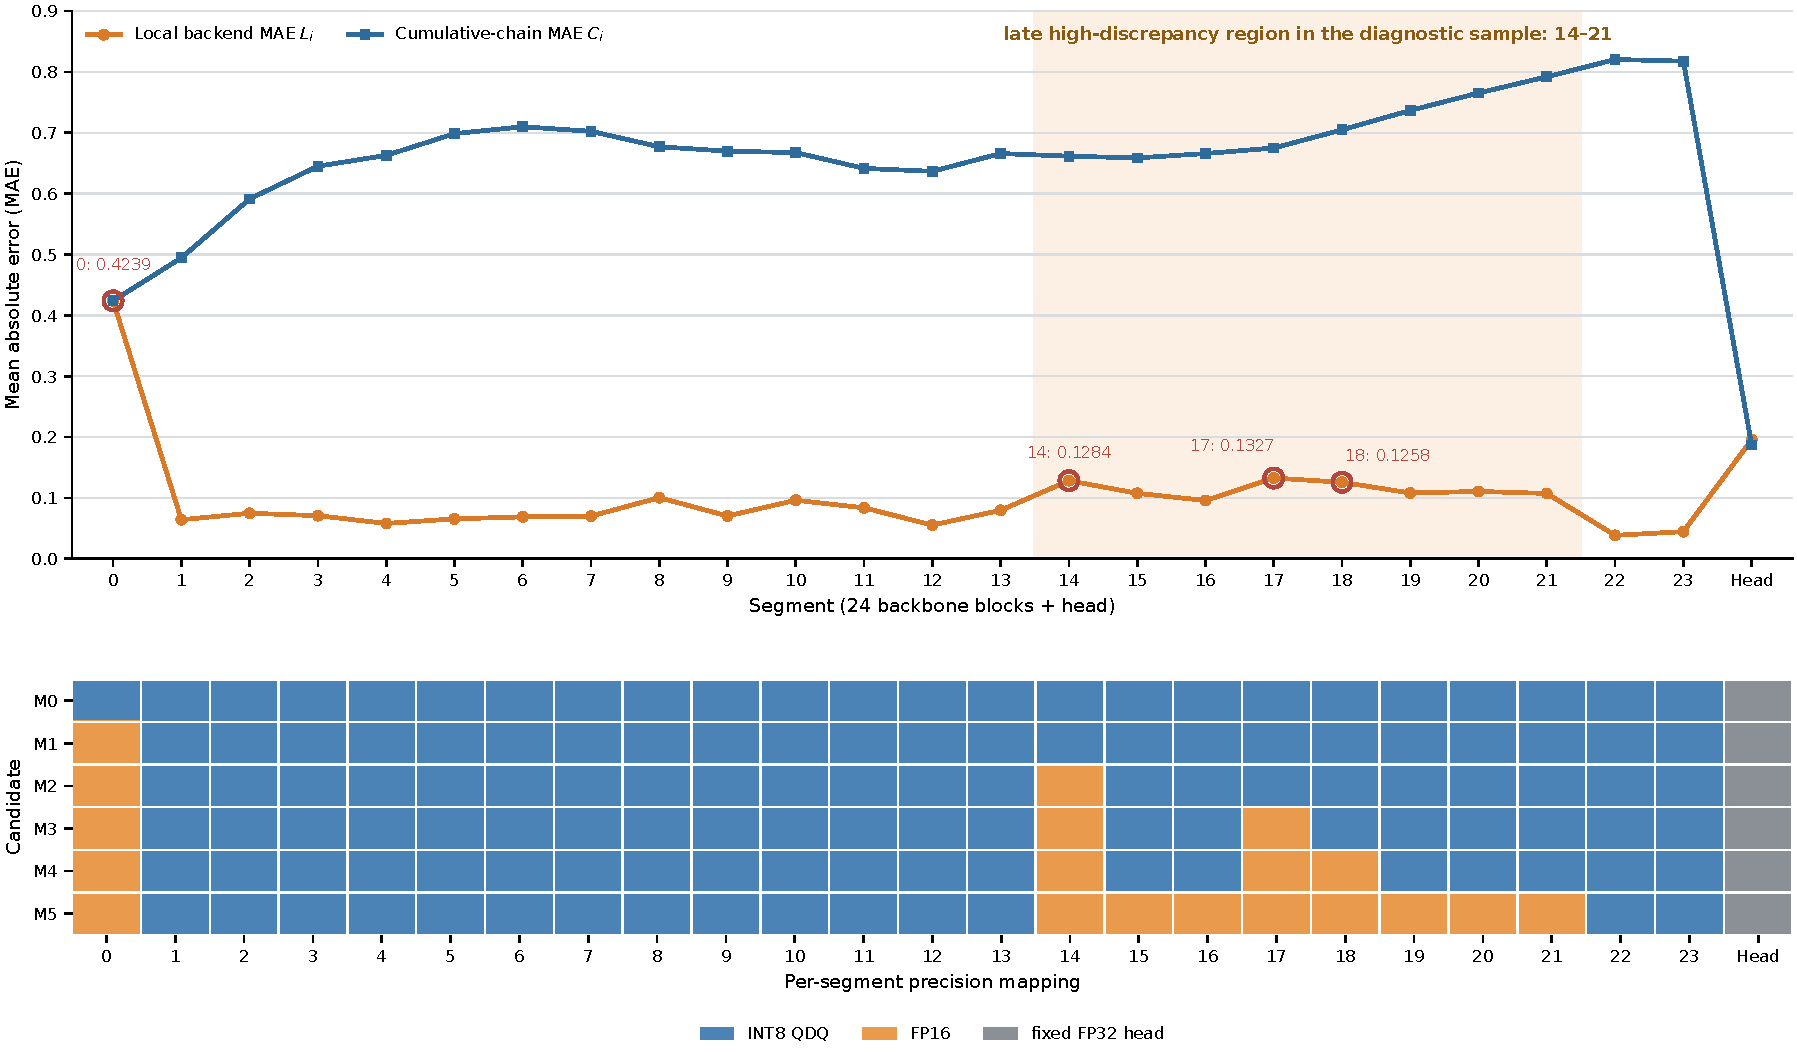
\includegraphics[width=0.98\textwidth]{figures/fig2_sensitivity_mapping_en.pdf}
\caption{CPU--MIGraphX backend-discrepancy profile for one diagnostic image and the resulting fixed M0--M5 precision maps. Circles mark the selected peaks used by M1--M4; M5 protects blocks 14--21. The profile is case-specific and does not estimate task-loss effects.}
\label{fig:sensitivity-map}
\end{figure*}

\subsection{Quantization and Model-Conversion Details}

The source checkpoint is the frozen Prithvi-EO-2.0-300M--UPerNet model trained with TerraTorch 1.2.8 (checkpoint SHA-256 beginning \texttt{59f031}). It was exported as an opset-17 FP32 ONNX graph with embedded input normalization, FP32 \texttt{image} input $[1,6,224,224]$, and FP32 \texttt{logits} output $[1,2,224,224]$. The export-side consistency check reported a maximum absolute difference of $4.768\times10^{-6}$. The exact PyTorch exporter version was not retained in the frozen sidecar and is therefore not inferred.

INT8 segments reuse immutable static-PTQ QDQ artifacts generated by ONNX Runtime quantization 1.26.0; this K100 study does not re-estimate scale or zero-point parameters. Activations and weights use signed 8-bit Q/DQ tensors (S8S8). Activations are asymmetric and weights symmetric; weights are per-channel, whereas activations are per-tensor. The quantizer-selected channel axes and resolved scale/zero-point tensor datatypes were not separately retained, so no axis or datatype is reconstructed here. MinMax calibration uses the first 64 examples, in dataset order, from the official training split after deterministic resize and the $10^{-4}$ input scale. No random augmentation or labels are used. Conv, MatMul, and Gemm form the whitelist; the backbone artifact selects one Conv and 144 MatMul nodes. LayerNorm, Softmax, residual Add, Resize, and other unselected operators remain on floating-point paths. Q/DQ pairs surround selected operator boundaries inside each segment, while the UPerNet head and all external segment interfaces remain FP32.

The frozen Full FP16 source was produced with \texttt{onnxconverter-common} 1.16.0 using FP32 external I/O; 332 initializers are FLOAT16 and 48 attention casts are patched in the conversion record. Extracted FP16 segments keep FP16 weights and activations, but compute LayerNorm statistics in explicit FP32 islands and place all casts inside the segment. ONNX Runtime 1.19.2 with the MIGraphX 5.1.0 Execution Provider compiles or loads each immutable ONNX segment as an MXR cache. Model and cache size/SHA identities, rather than an unrecorded command-line reconstruction, define the compiled artifacts used below.

\subsection{Evidence Tracks}

The experiment separates five evidence tracks.

\textit{Task track:} each candidate is evaluated on all 90 samples in three fresh processes. The task metrics above determine application acceptance.

\textit{Performance track:} after task acceptance, each candidate is measured with batch size 1, 30 warm-up runs, and three fresh processes with 100 timed runs per process. We report median, P95, P99, throughput, and the coefficient of variation (CV) of trial medians. A CV above 5\% prevents a formal speed claim.

\textit{Placement track:} every segment profile must contain positive MIGraphX events and zero CPU provider events. Inter-segment values remain on device.

\textit{Kernel track:} hipprof traces identify GEMM paths in each unique block artifact. I8II is expected for retained INT8 blocks and HBH for FP16 blocks. Q/DQ, casts, layout conversions, and copies are reported separately.

\textit{Operational track:} immutable deployment bundles are checked by manifest SHA-256, then tested through cold starts, forced recovery, cross-node execution, and 60-minute continuous runs.

A stricter CPU-versus-MIGraphX logits comparison is retained as a non-blocking diagnostic. It is not used to erase or override task-level evidence; its failure is reported explicitly in Section~\ref{sec:discussion}.

\section{Experimental Setup}
\label{sec:setup}

Experiments use two K100 nodes under the verified environment summarized in Table~\ref{tab:environment}. Container image identity, runtime fingerprint, model and cache hashes, input hashes, provider profiles, and raw latency arrays are frozen for each formal run. The placement tests disable implicit provider fallback; profiling evidence is parsed independently of session creation.

\begin{table*}[t]
\caption{Hardware, Software, and Measurement Environment}
\label{tab:environment}
\centering
\footnotesize
\begin{tabularx}{\textwidth}{>{\raggedright\arraybackslash}p{0.20\textwidth} X}
\toprule
Category & Verified configuration \\
\midrule
Accelerator & K100 AI accelerator; 2 nodes; 65,520 MiB device memory observed by \texttt{hy-smi}. \\
Host operating system & Ubuntu 20.04 LTS; Linux 5.4.0-216-generic. \\
Host memory & 62 GiB visible RAM. \\
Container image & Ubuntu 22.04.5; image \texttt{sha256:bdc7e817...17b01}. \\
Language/framework & Python 3.10.12; PyTorch 2.5.1; HIP 6.3.25405. \\
Compiler/runtime & DTK 25.04.2; MIGraphX 5.1.0+\texttt{das.opt1.dtk25042}; ONNX Runtime 1.19.2+\texttt{das.opt1.dtk25042}. \\
Operating policy & Batch 1; dynamic/auto performance mode observed; no competing K100 workload at preflight. \\
Timing method & Host \texttt{perf\_counter\_ns}; explicit I/O-binding input synchronization and final output synchronization. \\
Repetitions & 30 warm-ups; 3 fresh processes $\times$ 100 timed calls. \\
Model-only scope & Device-resident input OrtValue to device-resident logits. \\
End-to-end-logits scope & External FP32 input transfer through inference and final logits transfer to host. \\
Throughput definition & $N\times1000/\sum_j t_j$ samples/s for batch 1, with latency $t_j$ in ms. \\
Incremental VRAM definition & Separate fresh process; peak \texttt{mem\_info\_vram\_used} minus the median of 20 idle-baseline samples; 10-ms target polling. \\
Operations telemetry & Temperature, power, and VRAM sampled every 5 s during stability runs. \\
Input contract & FP32 $1\times6\times224\times224$; finite; fixed six-band order. \\
\bottomrule
\end{tabularx}
\end{table*}

For system performance, two timing scopes are distinguished. \textit{Model-only} starts with an input OrtValue resident on device and leaves logits resident. \textit{End-to-end-logits} includes the external input-to-logits path implemented by the common inference harness. A later paired comparison executes the complete M5 and Full FP16 bundles through the same public command-line interface and the same \texttt{K100BundleRunner.run} path.

The complete bundles accept a finite FP32 tensor of shape $1\times6\times224\times224$ and return FP32 logits of shape $1\times2\times224\times224$ plus a uint8 prediction map. Invalid shape, datatype, or non-finite inputs fail closed rather than being silently converted.

\subsection{Comparison Scope}

Table~\ref{tab:scope} defines the three comparison scopes used throughout the paper. Results are interpreted only within their stated scope; in particular, no precision-only speedup is inferred across different graph topologies or CLI paths.

\begin{table*}[t]
\caption{Comparison Scope and Valid Interpretation}
\label{tab:scope}
\centering
\small
\begin{tabular}{p{0.18\textwidth}p{0.23\textwidth}p{0.23\textwidth}p{0.20\textwidth}}
\toprule
Scope & Compared artifacts & Controlled interface & Allowed interpretation \\
\midrule
Topology matched & 25-segment FP32 versus M0--M5 & Same 25-session, device-resident OrtValue topology & Segmented-system latency and repeatability \\
Same-CLI & Final M5 bundle versus monolithic Full FP16 & Same fixed input and \texttt{K100BundleRunner.run} path & Production-style deployment decision, not isolated arithmetic effect \\
Storage & Logical ONNX+MXR capacity; complete bundle payload & Byte-count definitions reported separately & Capacity reduction only; no latency inference \\
\bottomrule
\end{tabular}
\end{table*}

\subsection{Reproducibility and Artifact Traceability}

Each formal result is linked to immutable ONNX and MXR SHA-256 identities, a fixed input hash, a container digest, a runtime fingerprint, and a configuration manifest. The retained project artifact package also contains raw latency arrays, provider profiles, kernel traces, complete-bundle manifests, static verification receipts, and exclusion ledgers. Failed launches are preserved separately and are never silently reclassified as accepted runs. These materials are retained with the project evidence package; the paper does not claim a public artifact release.

\section{Results}
\label{sec:results}

\subsection{Observed Backend-Discrepancy Distribution}

Table~\ref{tab:localization} reports the complete backend-discrepancy profile for the diagnostic image. Segment 0 is the earliest and largest local divergence: $L_0=0.4239$, relative $\ell_2=0.2978$, and $P_0=0$ because both chains start from the identical image. Blocks 14--21 form a later high-discrepancy region in this sample. Blocks 14, 17, and 18 are the clearest local peaks, while blocks 15, 16, and 19--21 remain moderately elevated. M2--M4 add the selected peaks; M5 protects the contiguous 14--21 region. This sequence records auditable engineering choices rather than estimating general block sensitivity.

\begin{table*}[t]
\caption{Per-Segment CPU--MIGraphX Backend-Discrepancy Localization on the Diagnostic Image}
\label{tab:localization}
\centering
\scriptsize
\begin{tabular}{crrrrl@{\qquad}crrrrl}
\toprule
Seg. & $L_i$ MAE & Local max & Rel. $\ell_2$ & $C_i$ MAE & Precision role & Seg. & $L_i$ MAE & Local max & Rel. $\ell_2$ & $C_i$ MAE & Precision role \\
\midrule
\textbf{0} & \textbf{0.4239} & \textbf{3.5917} & \textbf{0.2978} & 0.4239 & M1--M5 FP16 & 13 & 0.0797 & 0.4972 & 0.0507 & 0.6658 & INT8 \\
1 & 0.0642 & 1.4324 & 0.0459 & 0.4944 & INT8 & \textbf{14} & \textbf{0.1284} & 0.7954 & \textbf{0.0815} & 0.6615 & M2--M5 FP16 \\
2 & 0.0749 & 0.9584 & 0.0478 & 0.5913 & INT8 & 15 & 0.1076 & 0.5345 & 0.0663 & 0.6586 & M5 FP16 \\
3 & 0.0709 & 1.1014 & 0.0440 & 0.6450 & INT8 & 16 & 0.0958 & 0.9325 & 0.0587 & 0.6658 & M5 FP16 \\
4 & 0.0581 & 2.6298 & 0.0396 & 0.6628 & INT8 & \textbf{17} & \textbf{0.1327} & 1.2882 & \textbf{0.0807} & 0.6749 & M3--M5 FP16 \\
5 & 0.0656 & 0.7842 & 0.0409 & 0.6985 & INT8 & \textbf{18} & \textbf{0.1258} & 0.8274 & \textbf{0.0731} & 0.7048 & M4--M5 FP16 \\
6 & 0.0689 & 0.6987 & 0.0421 & 0.7098 & INT8 & 19 & 0.1081 & 0.8140 & 0.0616 & 0.7366 & M5 FP16 \\
7 & 0.0702 & 0.7861 & 0.0418 & 0.7023 & INT8 & 20 & 0.1107 & 0.6298 & 0.0622 & 0.7653 & M5 FP16 \\
8 & 0.1005 & 0.6774 & 0.0621 & 0.6770 & INT8 & 21 & 0.1074 & 0.6207 & 0.0582 & 0.7919 & M5 FP16 \\
9 & 0.0703 & 0.7109 & 0.0440 & 0.6697 & INT8 & 22 & 0.0386 & 0.2541 & 0.0199 & 0.8203 & INT8 \\
10 & 0.0963 & 1.7752 & 0.0609 & 0.6673 & INT8 & 23 & 0.0446 & 0.4270 & 0.0190 & 0.8176 & INT8 \\
11 & 0.0838 & 0.7812 & 0.0542 & 0.6414 & INT8 & Head & 0.1957 & 0.7799 & 0.1174 & 0.1871 & fixed FP32 \\
12 & 0.0554 & 1.0831 & 0.0401 & 0.6366 & INT8 & & & & & & \\
\bottomrule
\end{tabular}
\vspace{2pt}
\parbox{0.96\textwidth}{\scriptsize $L_i$: local same-input provider MAE; $C_i$: cumulative chain MAE. Bold rows are selected diagnostic peaks used by M1--M4. M5 additionally protects blocks 15, 16, and 19--21. These backend discrepancies are not pure quantization error or task-loss sensitivity; host-staged diagnostic timings are not performance evidence.}
\end{table*}

Third, neither local nor cumulative error is monotonic with depth. Blocks 22 and 23 have the two smallest local relative $\ell_2$ errors (0.0199 and 0.0190), yet their cumulative MAEs remain above 0.81 because they inherit earlier drift. Conversely, the cumulative error decreases at blocks 7--13 even when a nonzero local error is added. Residual addition, normalization, attention mixing, and MLP projections can rotate, attenuate, or amplify an existing perturbation; errors are vectors rather than nonnegative scalars that must add at every layer.

The local maximum must be read with MAE and relative $\ell_2$. Block 4 has a 2.6298 maximum but a 0.0581 MAE, indicating a sparse outlier rather than broad distortion. Block 14 has a smaller maximum but larger MAE and relative $\ell_2$, making it a stronger case-specific candidate for FP16 protection. The FP32 head exhibits a high local provider discrepancy, but its cumulative output MAE falls to 0.1871 after mapping multi-scale features to two logits. It is handled by the separate fpn4-barrier compatibility repair and is not labeled as a generally sensitive backbone layer.

\subsection{Strict Cross-Provider Logit Diagnostic}

Table~\ref{tab:strict-logits} retains the predefined single-image CPU-versus-MIGraphX diagnostic for the same frozen artifact and FP32 output logits. Its predefined strict cross-provider diagnostic tolerances are MAE $\leq10^{-3}$, maximum absolute error $\leq5\times10^{-2}$, and pixel-class agreement $\geq99.9\%$. These thresholds diagnose tight cross-provider interchangeability and are separate from the 90-image application-level segmentation criteria.

\begin{table*}[t]
\caption{Strict CPU--MIGraphX Logit Diagnostic on One Frozen Real Input}
\label{tab:strict-logits}
\centering
\small
\begin{tabular}{lrrrll}
\toprule
Artifact & MAE & Max abs. & Class agreement & Predefined tolerance & Status \\
\midrule
Full FP16 & 0.003715 & 0.013458 & 100.0000\% & $10^{-3}/5\!\times\!10^{-2}/99.9\%$ & failed (MAE) \\
M0 & 0.110935 & 0.609328 & 99.9960\% & same & failed \\
M1 & 0.126587 & 0.473313 & 100.0000\% & same & failed \\
M2 & 0.094231 & 0.407406 & 100.0000\% & same & failed \\
M3 & 0.104744 & 0.387089 & 100.0000\% & same & failed \\
M4 & 0.108455 & 0.393831 & 100.0000\% & same & failed \\
M5 & 0.092546 & 0.388980 & 100.0000\% & same & failed \\
\bottomrule
\end{tabular}
\end{table*}

The diagnostic failure remains permanent in this evidence record. It prevents claims of tight logit equivalence or calibrated cross-provider interchangeability, but it is not an application-level blocking criterion because deployment acceptance uses the frozen 90-image segmentation metrics and operational checks.

\subsection{Task Utility}

Table~\ref{tab:task} reports the frozen 90-image results. FP32 is reproduced exactly by the topology-matched baseline. Full FP16 changes mIoU by $-0.0131$ pp. All mixed configurations satisfy the fixed application criteria in three independent evaluation processes, with zero run-to-run metric span. M4 has the highest measured mixed-precision mIoU and Water IoU; M5 is slightly lower under this fixed protocol. These three process-level repetitions establish execution repeatability, not scene-level confidence or statistical significance.

\begin{table*}[t]
\caption{Task Metrics on the Fixed 90-Image Test Set}
\label{tab:task}
\centering
\small
\resizebox{\textwidth}{!}{%
\begin{tabular}{lccccccl}
\toprule
Variant & mIoU & Water IoU & Boundary Water IoU & Pixel Acc. & Agreement & Backbone blocks (FP32/FP16/INT8) & Task status \\
\midrule
FP32 & 0.860587 & 0.757838 & 0.362581 & 0.967110 & 100.0000\% & 24/0/0 & reference \\
Full FP16 & 0.860456 & 0.757588 & 0.361931 & 0.967094 & 99.9812\% & 0/24/0 & passed \\
M0 & 0.859288 & 0.755400 & 0.361058 & 0.966947 & 99.7071\% & 0/0/24 & passed \\
M1 & 0.860324 & 0.757386 & 0.362813 & 0.967077 & 99.8789\% & 0/1/23 & passed \\
M2 & 0.860044 & 0.756883 & 0.362193 & 0.967050 & 99.8731\% & 0/2/22 & passed \\
M3 & 0.860228 & 0.757201 & 0.362100 & 0.967065 & 99.8767\% & 0/3/21 & passed \\
M4 & 0.860371 & 0.757470 & 0.362530 & 0.967085 & 99.8753\% & 0/4/20 & passed \\
M5 & 0.860272 & 0.757295 & 0.362517 & 0.967029 & 99.8781\% & 0/9/15 & passed \\
\bottomrule
\end{tabular}
}
\parbox{0.98\textwidth}{\footnotesize The UPerNet head is FP32 for FP32 and M0--M5. Full FP16 follows its formally deployed monolithic compatibility graph: internal FP16 parameters/activations with FP32 islands and FP32 external I/O. All rows aggregate the same 90 images and 3,927,398 valid pixels.}
\end{table*}

The transition from M0 to M1 recovers most of the observed task degradation, consistent with protecting the high-discrepancy first segment in this case. Later FP16 substitutions do not produce a monotonic task-metric sequence. The M4--M5 differences are fixed-protocol descriptive differences only; no significance test or scene-level confidence interval is available.

Figure~\ref{fig:flood-qualitative} gives spatial context for the aggregate metrics. In the sparse-water scene, all three execution paths miss most of the small isolated water regions. In the moderate- and extensive-water scenes, the dominant false-positive and false-negative pixels lie along narrow shorelines and fragmented margins, while Full FP16 and M5 preserve the large-scale water geometry close to the matched FP32 output. These examples illustrate the error morphology but do not constitute an additional accuracy estimate.

\subsection{Logical Capacity and Compression}

Table~\ref{tab:capacity} reports executable-model and compiled-cache capacity. The segmented FP32 denominator is the sum of 25 ONNX files and 25 MXR caches, totaling 2,691,090,617 bytes (2566.424 MiB); M0--M5 use the same 25-segment accounting. Full FP16 uses its formally deployed monolithic ONNX and one paired MXR cache. For candidate $i$, the saved capacity is $S_{\mathrm{FP32}}-S_i$, the reduction is $(1-S_i/S_{\mathrm{FP32}})\times100\%$, and the compression ratio is $S_{\mathrm{FP32}}/S_i$. Full FP16 occupies 1284.756 MiB, corresponding to a 49.940\% reduction and 1.998$\times$ compression. M0 is the smallest candidate at 763.951 MiB (3.359$\times$), while M5 retains more FP16 blocks and occupies 981.759 MiB (2.614$\times$). Thus, protecting additional high-discrepancy blocks in the diagnostic sequence progressively trades storage for task accuracy, but every mixed candidate still reduces the segmented FP32 logical payload by more than 61\%.

\begin{table*}[t]
\caption{Logical ONNX+MXR Capacity and Compression Relative to the Same-Topology FP32 Baseline}
\label{tab:capacity}
\centering
\small
\resizebox{\textwidth}{!}{%
\begin{tabular}{llrrrrrr}
\toprule
Variant & Backbone precision map & ONNX (MiB) & MXR (MiB) & Total (MiB) & Saved vs. FP32 (MiB) & Reduction & Compression ratio \\
\midrule
FP32 & 24 FP32 & 1218.134 & 1348.290 & 2566.424 & 0.000 & 0.000\% & 1.000$\times$ \\
Full FP16 & monolithic FP16 & 609.370 & 675.386 & 1284.756 & 1281.668 & 49.940\% & 1.998$\times$ \\
M0 & 0 FP16 + 24 INT8 & 350.990 & 412.960 & 763.951 & 1802.473 & 70.233\% & 3.359$\times$ \\
M1 & 1 FP16 + 23 INT8 & 364.016 & 425.362 & 789.378 & 1777.046 & 69.242\% & 3.251$\times$ \\
M2 & 2 FP16 + 22 INT8 & 375.936 & 437.417 & 813.353 & 1753.071 & 68.308\% & 3.155$\times$ \\
M3 & 3 FP16 + 21 INT8 & 387.856 & 449.666 & 837.522 & 1728.903 & 67.366\% & 3.064$\times$ \\
M4 & 4 FP16 + 20 INT8 & 399.776 & 461.913 & 861.689 & 1704.735 & 66.425\% & 2.978$\times$ \\
M5 & 9 FP16 + 15 INT8 & 459.375 & 522.384 & 981.759 & 1584.665 & 61.746\% & 2.614$\times$ \\
\bottomrule
\end{tabular}
}
\end{table*}

These figures describe one executable configuration's logical ONNX+MXR payload and exclude the container image, Python/runtime dependencies, filesystem allocation effects, and hard-link sharing across candidates. Full FP16 is monolithic, whereas FP32 and M0--M5 are segmented; the row is therefore a storage comparison, not a topology-matched execution comparison. These values are also not interchangeable with the complete deployment-bundle figures reported later.

\begin{figure}[!t]
\centering
\makebox[\columnwidth][c]{%
  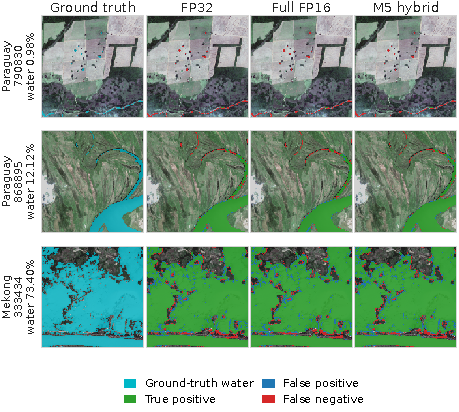
\includegraphics[width=0.96\columnwidth]{figures/fig_flood_qualitative_en.pdf}%
}
\caption{Qualitative flood-water delineation on three fixed test scenes. Scenes are selected independently of model accuracy at the 25th, 75th, and 95th percentiles of valid-pixel ground-truth water coverage among nonempty masks. Cyan marks ground-truth water. Prediction rows overlay true positives in green, false positives in blue, and false negatives in red on the RED--GREEN--BLUE composite. This visualization is illustrative and does not replace the 90-image metrics in Table~\ref{tab:task}.}
\label{fig:flood-qualitative}
\end{figure}

Figure~\ref{fig:tradeoff} separates logical capacity from topology-matched latency. The monolithic Full FP16 latency is shown only as an independent callout because it was measured under the final same-CLI single-session scope.

\begin{figure*}[t]
\centering
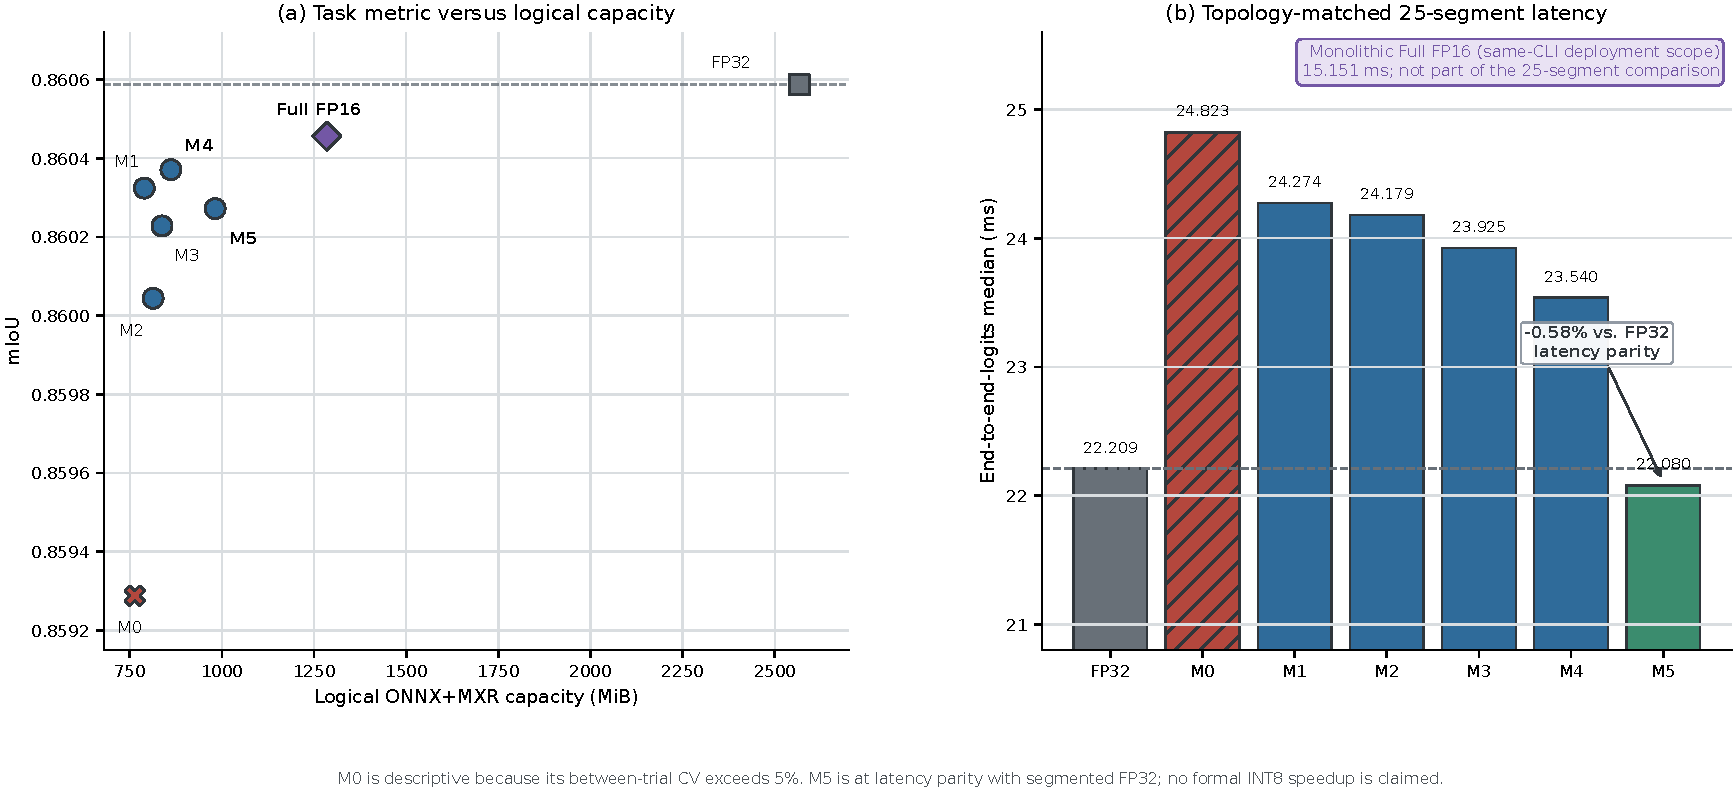
\includegraphics[width=0.98\textwidth]{figures/fig3_tradeoff_en.pdf}
\caption{Two comparison scopes. (a) mIoU versus logical ONNX+MXR capacity for FP32, Full FP16, and M0--M5. (b) topology-matched end-to-end-logits latency for 25-segment FP32 and M0--M5; Full FP16 is an independent same-CLI callout. No cross-scope precision-only speedup is implied.}
\label{fig:tradeoff}
\end{figure*}

\subsection{Same-Topology Performance}

Table~\ref{tab:performance} compares only the matched 25-segment FP32 denominator and M0--M5. M1--M4 are slower than FP32. M5 has a 22.080 ms end-to-end-logits median versus 22.209 ms for FP32, approximately 0.58\% lower. We describe this as latency parity with segmented FP32 and make no formal INT8 speedup claim. The original M0 model-only run has a 6.47\% trial-median CV and remains marked unstable; a later confirmation does not overwrite that frozen status.

\begin{table*}[t]
\caption{Topology-Matched Performance of the 25-Segment Configurations}
\label{tab:performance}
\centering
\small
\resizebox{\textwidth}{!}{%
\begin{tabular}{lcccccc}
\toprule
Variant & Model-only median (ms) & End-to-end-logits median (ms) & Speed factor $T_{\mathrm{FP32}}/T_{\mathrm{variant}}$ & Incremental VRAM (GiB) & CV status & Interpretation \\
\midrule
FP32 & 21.349 & 22.209 & 1.000$\times$ & 19.230 & passed & denominator \\
M0 & 24.136 & 24.823 & 0.895$\times$ & 17.200--17.400 & unstable & maximum compression \\
M1 & 23.550 & 24.274 & 0.915$\times$ & 17.200--17.400 & passed & compact stable \\
M2 & 23.411 & 24.179 & 0.919$\times$ & 17.200--17.400 & passed & slower than FP32 \\
M3 & 23.118 & 23.925 & 0.928$\times$ & 17.200--17.400 & passed & slower than FP32 \\
M4 & 22.829 & 23.540 & 0.944$\times$ & 17.200--17.400 & passed & accuracy-oriented \\
M5 & 21.339 & 22.080 & 1.006$\times$ & 17.200--17.400 & passed & parity; no speed claim \\
\bottomrule
\end{tabular}
}
\parbox{\textwidth}{\footnotesize Note: all rows use the matched 25-segment resident-session protocol, batch 1, 30 warm-ups, and three fresh processes with 100 timed runs each. A factor above 1 denotes lower median latency than segmented FP32; below 1 denotes higher latency. The 1.006$\times$ M5 value is latency parity, not a formal INT8 speedup.}
\end{table*}

The fixed configurations expose different measured trade-offs. M0 is the maximum-compression candidate but retains its unstable timing status. M1 is the first compact configuration that recovers most of M0's task degradation and satisfies the timing-stability criterion. M4 is the accuracy-oriented mixed-precision point, and M5 is the segmented-latency-oriented point and final storage-oriented deployment alternative. Full FP16 is evaluated separately against M5 in Table~\ref{tab:cli}; it is not a 25-segment baseline.

\subsection{Kernel and Placement Evidence}

All 25 segments in the accepted candidates show positive MIGraphX events and zero CPU provider events. Kernel analysis covers 33 de-duplicated traces---24 INT8 identities and nine FP16 identities---which expand to 144 candidate--block mappings. Every retained INT8 block observes the expected I8II GEMM path, and every FP16 block observes the HBH path.

The traces provide execution detail beyond an ONNX datatype inspection, but remain block-level evidence. The FP32 head, LayerNorm islands, Q/DQ operations, casts, layout conversions, and copies remain part of the full pipeline. Consequently, the traces provide evidence that integer GEMMs are realized where intended; they do not establish that every operator is integer or that the complete model must be faster.

\subsection{Deployment Payload and Same-CLI Comparison}

The M5 bundle contains 74 payload files totaling 1,032,911,027 bytes, whereas the Full FP16 bundle contains 19 payload files totaling 1,349,558,844 bytes. Thus M5 reduces the complete deployment payload by 316,647,817 bytes, or 23.463\%. This complete-bundle scope includes executable artifacts, manifests, tools, and fixed verification data; it is distinct from both ONNX-only compression and the ONNX+MXR logical capacity in Table~\ref{tab:capacity}.

The final paired benchmark uses the same public CLI, fixed input, runner implementation, and $3\times100$ protocol for both bundles. As shown in Table~\ref{tab:cli}, M5 is slower than Full FP16 even though it is smaller and contains verified INT8 GEMMs. This production-style comparison informs the deployment recommendation, but it cannot isolate arithmetic precision from graph topology.

\begin{table}[t]
\caption{Production-Style Same-CLI Comparison of the Final Deployment Bundles}
\label{tab:cli}
\centering
\footnotesize
\begin{tabular}{lrrrr}
\toprule
Bundle & Median & P95 & P99 & Throughput \\
 & (ms) & (ms) & (ms) & (samples/s) \\
\midrule
M5 & 26.309 & 28.518 & 30.744 & 37.641 \\
Full FP16 & 15.151 & 15.552 & 17.594 & 65.900 \\
\bottomrule
\end{tabular}
\vspace{2pt}
\parbox{0.96\columnwidth}{\footnotesize M5/FP16 median-latency ratio: 1.7364; M5 is 73.642\% slower. Trial-median CV is 0.413\% for M5 and 0.086\% for FP16. This same-CLI comparison combines precision and topology effects; it is not a precision-only hardware ratio.}
\end{table}

\balance
\subsection{Operational Validation}

Both immutable bundles pass full static verification, including manifest and payload hashes, runtime fingerprint, input/output contract, and fixed-vector prediction checks. Each passes five cold starts and three forced termination-and-reload cycles. Median session-load times are 8.883 s for M5 and 10.086 s for FP16; median total runner initialization times are 10.281 s and 11.570 s, respectively. These are startup measurements and are not used as steady-state throughput evidence.

Both bundles pass smoke tests on K100-2 and K100-3 with the formal launch environment attested outside the container. In the 60-minute runs, M5 completes 123,106 inferences and FP16 completes 193,634. Each run records 720 telemetry samples and zero crashes, inference errors, non-finite outputs, or fixed-sample prediction drift. M5 operates over 41--67$^{\circ}$C and 108--217 W, while FP16 operates over 43--59$^{\circ}$C and 109--202 W. Two earlier invalid K100-3 launch attempts and one attestation-tool failure are preserved in exclusion ledgers; none counts toward acceptance, and none reached a successful model inference.

\section{Discussion}
\label{sec:discussion}

\subsection{Interpretation of the Backend-Discrepancy Diagnosis}

The M0-to-M1 change is consistent with protecting the first high-discrepancy segment in the diagnostic image. Blocks 14--21 form a second region in that same profile, but neither local nor cumulative discrepancy is monotonic. Residual addition, normalization, attention mixing, and MLP projections can attenuate, rotate, or amplify an existing perturbation, while UPerNet consumes multiple intermediate features. The profile is therefore useful for constructing an auditable sequence, not for declaring blocks 0 and 14--21 universally sensitive. M0, M1, M4, and M5 should be read as fixed maximum-compression, compact-stable, accuracy-oriented, and segmented-latency-oriented ablations, respectively.

\subsection{Why Verified INT8 Kernels Do Not Guarantee End-to-End Speedup}

M5 satisfies the block-level I8II requirement, yet it is slower than the monolithic Full FP16 deployment under the same CLI. The observation is consistent with the combined effects of multi-session dispatch, segment boundaries, Q/DQ operations, FP32 interfaces, casts, layout transformations, the FP32 head, and remaining floating-point operators. Their individual contributions are not isolated here, so no numerical fraction of the latency gap is assigned to one source. Realized INT8 kernels are therefore necessary evidence about arithmetic execution, but not sufficient evidence of application-level acceleration.

\subsection{Deployment Implications}

Task-metric preservation and strict logit equivalence answer different questions. All configurations satisfy the fixed application criteria, whereas the historical strict CPU/MIGraphX logit diagnostic remains failed for the INT8 and mixed artifacts. That failure is not overwritten by task acceptance. Applications that depend on calibrated logits or tight cross-provider reproduction require further validation. For the present segmentation deployment, immutable manifests, fixed I/O contracts, placement profiles, cold starts, recovery, cross-node execution, and 60-minute runs provide the operational evidence used here. The recorded power and temperature ranges are operational observations, not controlled energy-efficiency measurements.

\subsection{Threats to Validity}

\textit{Internal validity:} calibration uses 64 images from the official training split, but no independent split is reserved for configuration selection. One public-test-split image informed M0--M5 construction and is included in the same 90-image evaluation, so configuration-selection bias is possible. The result is a fixed deployment-validation case study, not an unbiased held-out estimate of configuration generalization.

\textit{Construct validity:} CPU--MIGraphX differences from the same frozen artifacts are backend discrepancies, not pure FP32-to-INT8 quantization error or task-loss sensitivity. I8II/HBH traces identify block-level GEMM paths, not the datatype of every operation. Logical ONNX+MXR capacity and complete bundle payload are different storage constructs, and strict logit equivalence is distinct from task-metric preservation.

\textit{External validity:} the evidence covers one Prithvi checkpoint, one flood-segmentation task, one split, batch size 1, and one K100 software stack. The observed discrepancy pattern and timing trade-offs may change with scenes, checkpoints, tasks, compiler versions, or accelerators.

\textit{Conclusion validity:} three fresh processes characterize run-to-run repeatability; they do not provide scene-level confidence intervals or statistical-significance tests. Small M4--M5 task differences are descriptive, and the approximately 0.58\% M5--FP32 median difference is reported as latency parity rather than acceleration. The present evidence is sufficient for the stated deployment decision under the frozen protocol, but not for a general mixed-precision optimization claim.

\subsection{Final Deployment Recommendation}

Full FP16 is the speed-oriented primary deployment for the evaluated stack: it retains near-FP32 task metrics and is faster than M5 under the same external CLI. M5 is a storage-oriented deployable alternative because it passes the task, placement, kernel, recovery, cross-node, and stability checks while reducing complete bundle payload by 23.463\%. M4 remains the accuracy-oriented mixed-precision ablation; M1 is the compact stable/first-recovery ablation; and M0 records maximum compression with unstable timing. This recommendation does not imply that FP16 is universally preferable or that M5 is a general mixed-precision policy.

\section{Conclusion}

For the evaluated Prithvi checkpoint and K100 software stack, auditable deployment requires consistent evidence from task metrics, provider placement, realized kernels, matched timing, and operations. The diagnosis-informed M5 configuration preserves task utility, reaches latency parity with segmented FP32 (approximately 0.58\% lower median latency), and reduces complete bundle payload by 23.463\%, but it neither establishes strict cross-provider logit equivalence nor a formal INT8 speedup. Verified I8II kernels do not guarantee application-level acceleration: M5 is 73.642\% slower than Full FP16 under the same production-style CLI. Full FP16 is therefore the speed-oriented primary deployment, while M5 remains a smaller storage-oriented alternative. These conclusions define a deployment decision under the frozen protocol, not a general precision policy or universal block-sensitivity pattern.

\bibliographystyle{IEEEtran}
\bibliography{references}

\end{document}
